\newcommand{\boundellipse}[3]% center, xdim, ydim
    {(#1) ellipse (#2 and #3)
}

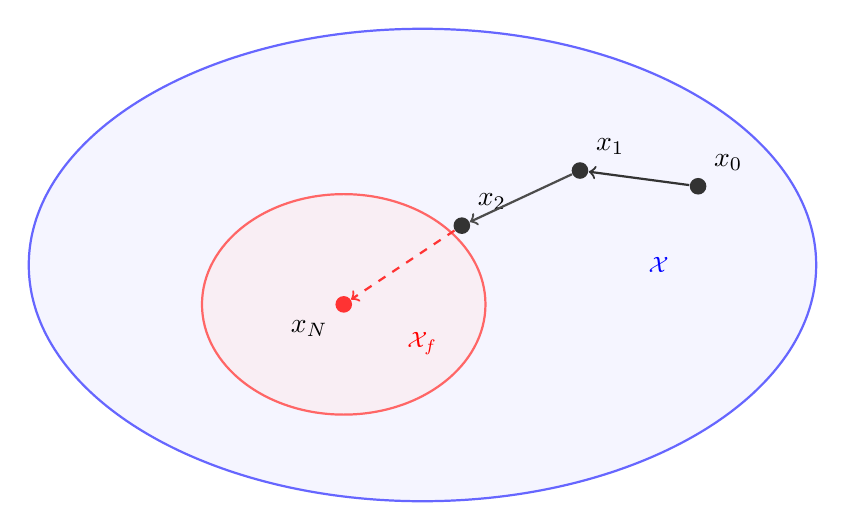
\begin{tikzpicture}[
    dot/.style={circle, fill=black!80, inner sep=1pt, minimum size=6pt},
    red-dot/.style={circle, fill=red!80, inner sep=1pt, minimum size=6pt}
]
    % State constraint set X (Large blue ellipse centered at 0,0)
    \fill[blue!10, fill opacity=0.4] \boundellipse{0,0}{5}{3};
    \draw[blue!60, thick] \boundellipse{0,0}{5}{3};
    \node[text=blue, font=\footnotesize] at (3, 0) 
        {$\mathcal{X}$};
    
    % Terminal set Xf (Smaller red ellipse shifted to the bottom-left)
    \fill[red!10, fill opacity=0.4] \boundellipse{-1,-0.5}{1.8}{1.4};
    \draw[red!60, thick] \boundellipse{-1,-0.5}{1.8}{1.4};
    \node[text=red, font=\footnotesize] at (0, -1) 
        {$\mathcal{X}_f$};

    % Nodes
    % Syntax: \node[Style, label=Position:Text] (Name) at (Koordinaten) {};
    \node[dot, label=above right:$x_0$]    (x0)  at (3.5, 1.0)  {};
    \node[dot, label=above right:$x_1$]    (x1)  at (2.0, 1.2)  {};
    \node[dot, label=above right:$x_2$]    (x2)  at (0.5, 0.5)  {};
    \node[red-dot, label=below left:$x_N$] (xN) at (-1.0, -0.5) {};

    % Automatically connect the nodes by their names (without typing coordinates!)
    \draw[->, black!80, thick] (x0) -- (x1);
    \draw[->, black!70, thick] (x1) -- (x2);
    \draw[->, red!80, thick, dashed] (x2) -- (xN);
    
\end{tikzpicture}